\section{Hardware Friendly Training}\label{sec:training}
In this section, we introduce our hardware-friendly training method using fixed point data and advanced pruning. The whole training process includes the following steps:
\begin{itemize}
  \item Train the model with full-precision activations, weights, gradients and errors.
  \item Prune the model. 
  \item Apply quantization to activations, weights, gradients and errors according to the last epoch of training.  
  \item Continue training the pruned model with fixed-point activations, weights, gradients and errors.
\end{itemize}
We will focus on pruning and data quantization in this section.

\subsection{Advanced Pruning}\label{sec:training:prune}

Pruning brings acceleration potential to training. By forcing part of the weights to zero, we reduce not only the computation in FP and EB phases, but also the computation in WG phases because the gradients to the zero weights are not needed. Traditional pruning is usually applied when the model is well trained. To increase the potential of acceleration, we choose to prune the model before the training process converges. We also use a structured pruning method for convolution layers to simplify the hardware design. We denote shape of weights as $(N, C, H, W)$. $N$ represents output channel, $C$ represents input channel, $H$ represents height, and $W$ represents width. The pruning method masks each $H\times W$ kernel as a whole if the L2-norm of the kernel is small. 

In this work, the pruning process is automatically done by pruning the kernels with the smallest L2-norms as long as the accuracy drop of the model is within a given range. To reduce the time for validation, pruning is done layer by layer and with a step of 10\% weights of each layer.

\begin{figure}[tb]
    \centering
    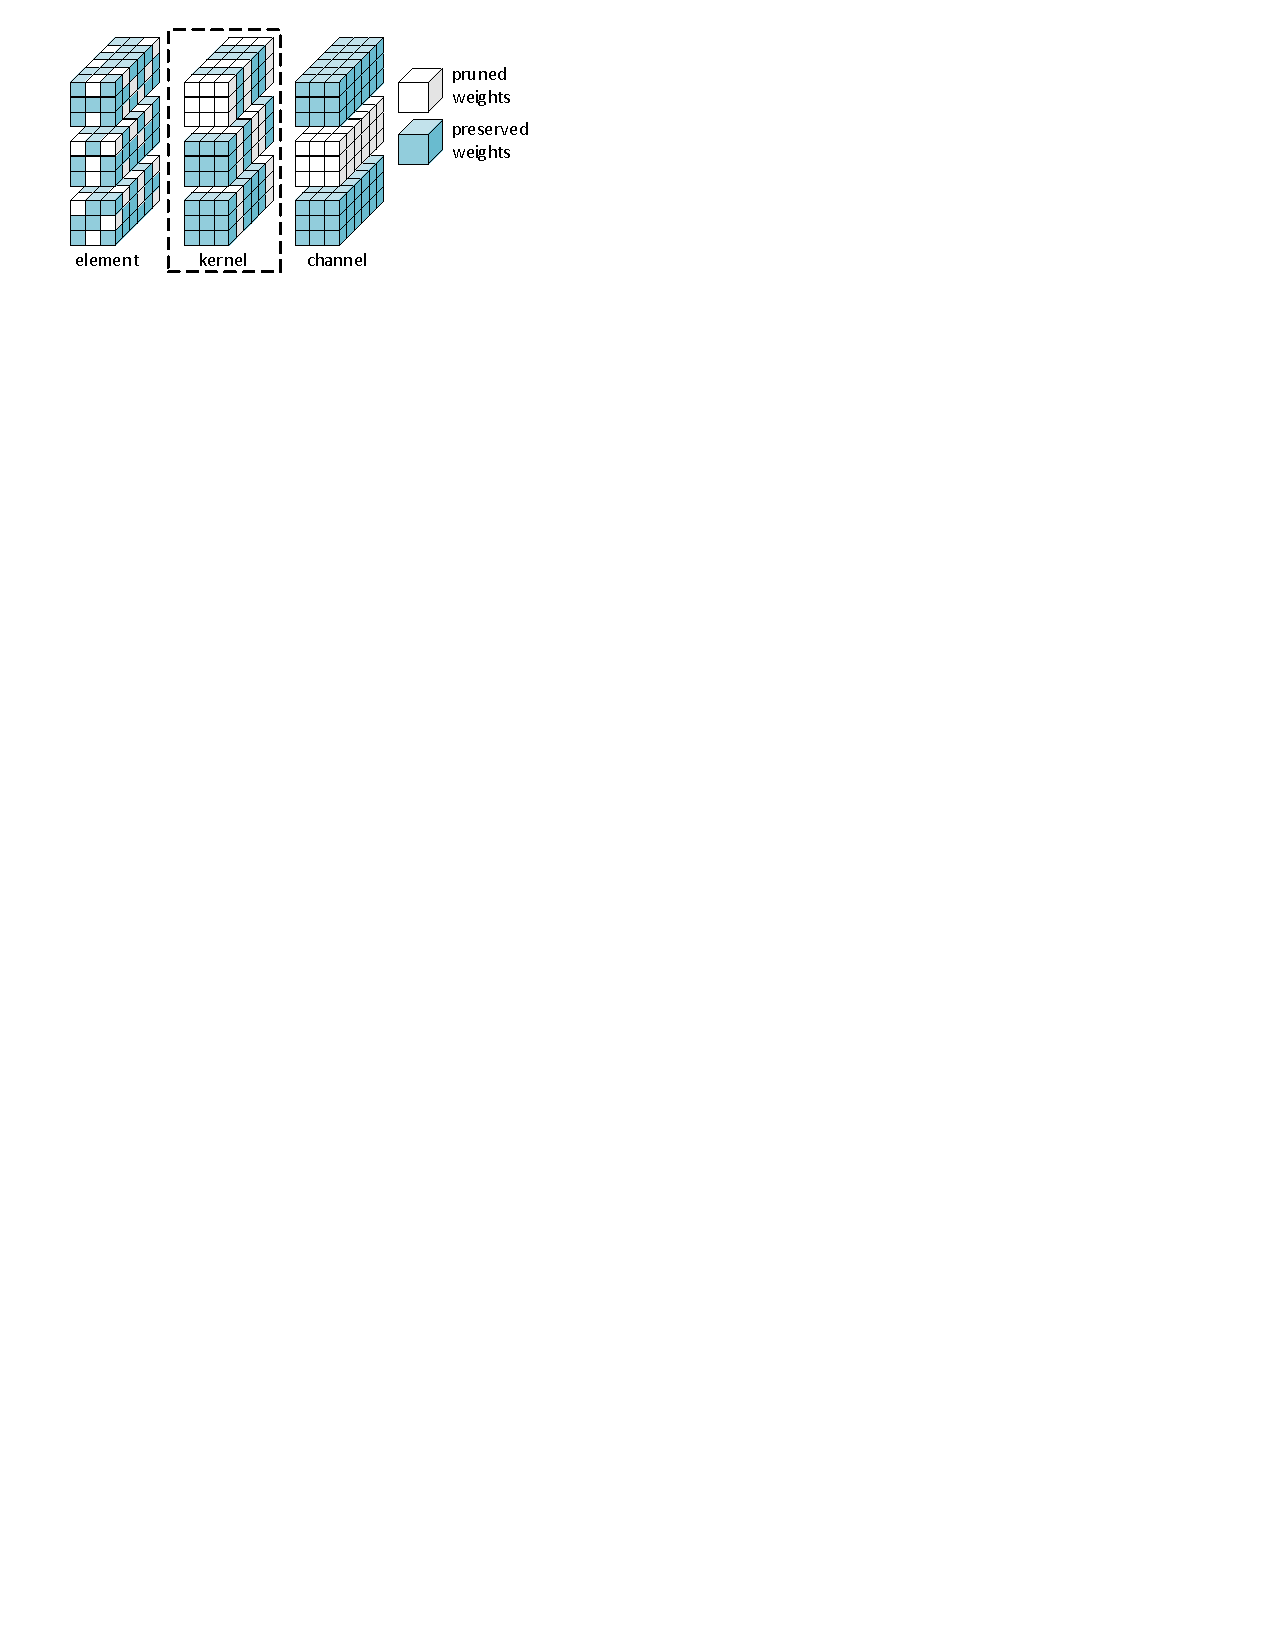
\includegraphics[width=0.9\columnwidth]{figures/prune.pdf}
    \caption{Illustration of the kernel-wise pruning}\label{fig:prune}
\end{figure}

\subsection{Data Quantization in Training}
Traditional CNN training relies on full-precision data, i.e. 32-bit floating point data, to guarantee a good training accuracy. However, using fixed-point data in training process can help increase the energy efficiency of training. For CNN inference, varies accelerators have been proposed with fixed point operations to increase energy efficiency. For training, using fixed point data usually suffers great model accuracy loss. Recent work~\cite{zhou2016dorefa} use narrow bit-width only for data storage in training process but have to convert the data to floating point to process addition and multiplication. In this paper, we propose a training process using both fixed point format for data storage and computation. 

In the proposed training process, every fixed-point number is represented with low bit-width (e.g. 8 bit in our implementation) together with a scaling factor. We keep a common scale for each fixed-point blob, where a blob can be the activation, weights, gradient or error of a layer. Directly using this data format will induce two problems.

The first problem is how to convert the original floating point data to the fixed point version. One choice is to use the dynamic range of each blob as the scaling factor. This strategy keeps the data precision to the best degree, but brings extra statistic and normalization operations for each data blob in each iteration. In this work, we execute floating-point training iterations to analyze the dynamic scale of each blob and keep the scale through the rest of training process. We choose the nearest $2^n$ as the scaling factor which means data normalization can be implemented with shift operations on fixed-point data.

The second problem is the trade-off between bit-width and training accuracy. Low bit-width simplifies operations and reduce the storage consumption, but also reduce the model accuracy. Consider the small learning rate and gradient vanishing, the updated value in each iteration is small, the scaling factor of weights can be much larger than that of gradients. We use a large bit-width (i.e. 32-bit) to represent both the weights and gradients but only use the MSBs of weights in FP and EB phases. Figure~\ref{fig:fixed_train} shows the proposed training example. All the MAC operations in FP, WG, and EB phases are executed with 8-bit fixed point data.  

\begin{figure}[tb]
  \centering 
  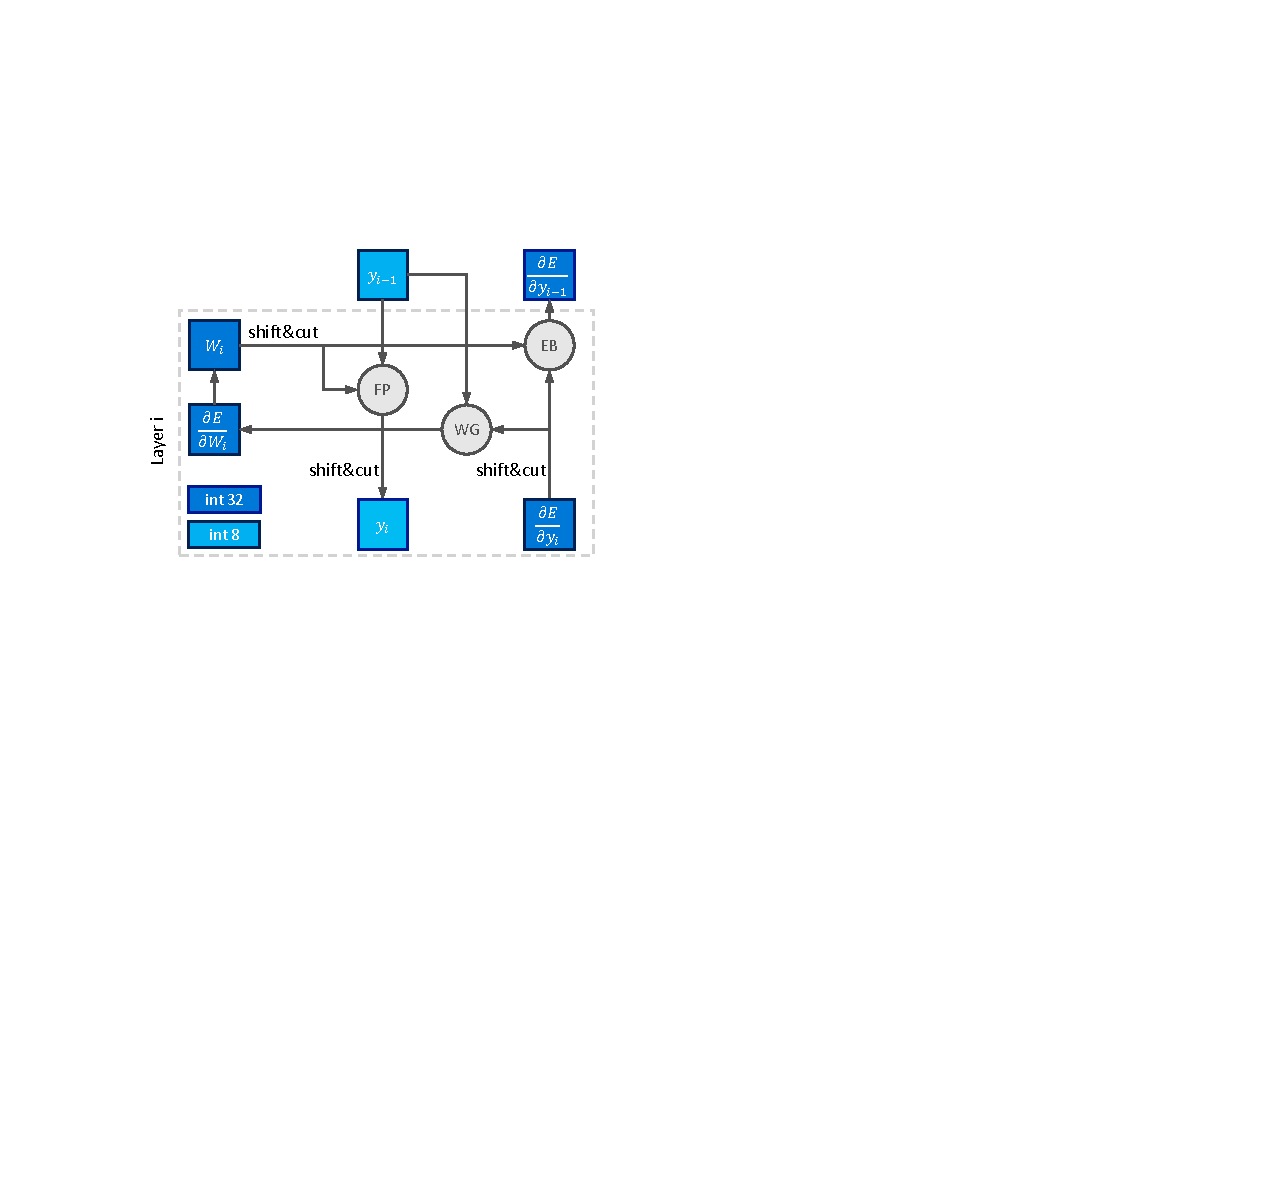
\includegraphics[width=0.9\columnwidth]{figures/fixed_train.pdf}
  \caption{Proposed hardware-friendly training process with fixed-point data. The weights are stored with long bit-width (32-bit in the figure) to make valid accumulation. The computations are processed with short bit-width (8-bit in the figure).}
  \label{fig:fixed_train}
\end{figure}


